%
% teil1.tex -- Brownische Bewegung
%
% (c) 2023 Lukas Reitemeier, OST Ostschweizer Fachhochschule
%
% !TEX root = ../../buch.tex
% !TEX encoding = UTF-8
%

\section{Brownsche Bewegung\label{brown:BrownBewegung}}
\rhead{Brownsche Bewegung}

\begin{figure}
	\centering
	\begin{minipage}{0.45\textwidth}
		\centering
		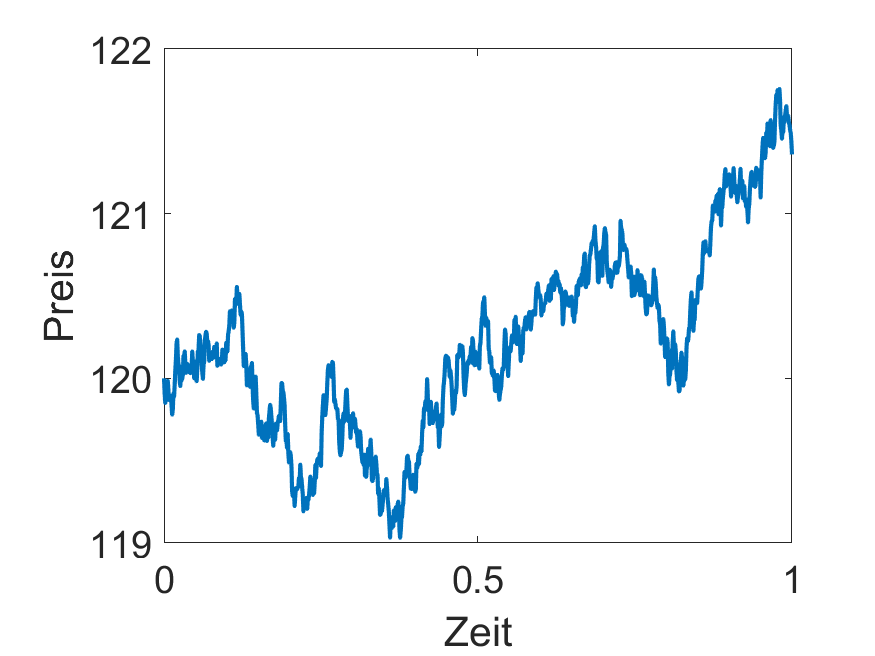
\includegraphics[width=\linewidth]{papers/brown/images/boersenKurs-simuliert.png}
		\caption{Simulierter Börsenkurs}
		\label{brown:1Dbrownian}
	\end{minipage}
	\hspace{0.05\linewidth}
	\begin{minipage}{0.45\textwidth}
		\centering
		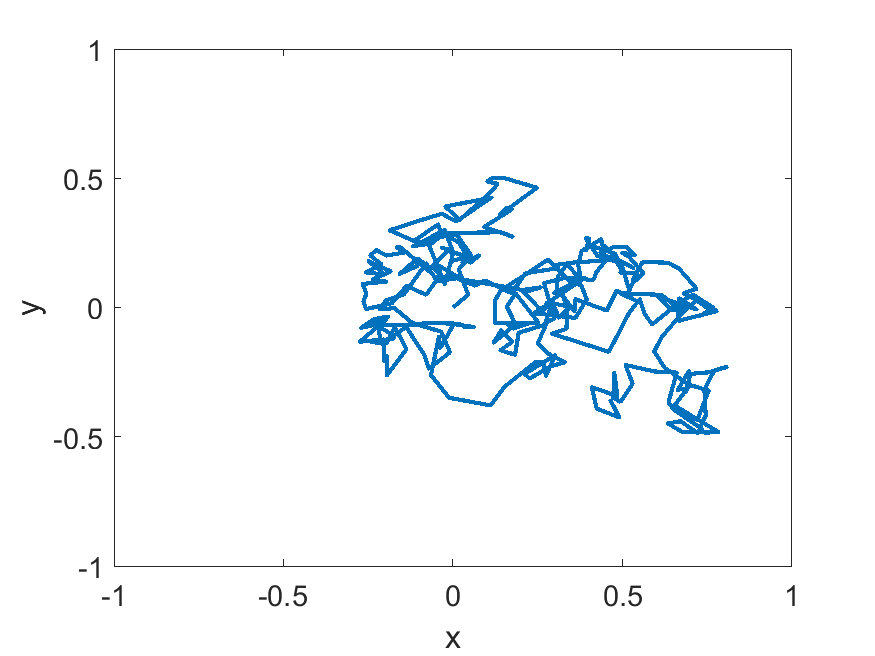
\includegraphics[width=\linewidth]{papers/brown/images/brownscheBewegung-simuliert.png}
		\caption{Simulierte brownsche Bewegung}
		\label{brown:2Dbrownian}
	\end{minipage}
\end{figure}

Als der schottische Botaniker Robert Brown im Jahr 1827 in sein Mikroskop schaute, beobachtete er kleine Pollenpartikel in einer Flüssigkeit. Er bemerkt, dass sich die Teilchen scheinbar zufällig bewegen, obwohl keine Kräfte auf die Teilchen einwirken. Eine Erklärung hatte Robert Brown zu diesem Zeitpunkt für das Verhalten nicht. Es dauerte fast ein Jahrhundert, bis Albert Einstein diese Beobachtung auf ein solides theoretisches Fundament stellte und so nutzbar machte. Er schloss darauf, dass die unregelmäßige Bewegung auf Kollisionen mit umgebenden Molekülen zurückzuführen ist, welche ständig in Bewegung sind. Albert Einstein entwickelte ein mathematische Theorie, mit welcher die beobachtete Bewegung durch stochastische Zusammenstöße von Molekülen erklärt werden kann. Weiter konnte er einen Zusammenhang zwischen den Messungen der Bewegung, der Bolzmann-Konstante und der  Avogadro-Zahl herstellen\footnote{Die Avogadro-Zahl $ A $ ist die Anzahl Teilchen (Atome oder Moleküle) welche in einem Mol einer Substanz enthalten sind. Die Boltzmann-Konstante $ k $ ist eine physikalische Konstante, die den Zusammenhang zwischen der thermischen Energie und der Temperatur eines Systems herstellt. Beide Konstanten sind miteinander verbunden durch die Gleichung $ k = \frac{R}{A} $, wobei $ R $ die allgemeine Gaskonstante ist.}. Dies hatte Auswirkungen auf das Verständnis von Materie, da dies einen direkten empirischen Beleg für die Existenz von Atomen und Moleküle lieferte --- die Atomhypothese wurde nicht nur bestätigt, sie wurde durch die brownsche Bewegung auch beobachtbar. Diese besagt, dass Materie aus diskreten unteilbaren Einheiten besteht, sprich einzelnen Atomen oder ganzen Molekülen. Man muss dazu sagen, dass es schon zuvor Indizien für deren Existenz gab, doch es fehlte am entscheidenden experimentellen Beweis.


Die \textit{Einstein-Smoluchowski-Gleichung} ist eine zentrale Gleichung in seiner Arbeit. Sie beschreibt die mittlere quadratische Verschiebung (\textit{mean square displacement})

\begin{equation}
	\mathrm{MSD} = 2nDt
\end{equation}

in Beziehung zur Diffusionskonstanten $ D $ , der Anzahl Raumdimensionen $ n $ und der Zeit $ t $. Die Avogadro-Zahl $ A $ kann indirekt über die \textit{Stokes-Einstein-Gleichung}, anhand von Messungen berechnet werden. Die Diffusionskonstante $ D $ wird dabei mittels des Radius der suspendierten Teilchen, der Boltzmann-Konstante  $ k $, der Temperatur $ T $ und der Viskosität $ \eta $ des umgebenden Mediums wie folgt berechnet:

\begin{equation}
	D = \frac{kT}{6\pi\eta r}
\end{equation}

$ r $ beschreibt dabei den Radius des suspendierten Teilchens. Die Boltzmann-Konstante $ k $ kann auch durch die allgemeine Gaskonstante $ R $ und die Avogadro-Zahl $ A $ ausgedrückt werden: $ k = R/A $, wodurch sich folgender Zusammenhang für die Avogadro-Zahl ergibt:

\begin{equation}
	A = \frac{R T}{D (6 \pi \eta r)}
\end{equation}

So ermöglichen die beiden Gleichungen einen experimentellen Ansatz zur Bestimmung der Avogadro-Zahl und ferner die quantitative Analyse einer brownschen Bewegung.

Die brownsche Bewegung kann relativ einfach mittels der Euler-Maruyama-Methode \ref{brown:Simulation} numerisch simuliert werden. Zugrunde liegt dabei der Wiener-Prozess \ref{brown:Rauschen:RandomWalkWiener}. Dieser liefert die zufälligen Veränderungen in X- und Y-Richtung. Werden die einzelnen Zeitschritte mit Linien verbunden, ergibt sich das Bild einer typischen brownschen Bewegung, wie dies in der Abbildung \ref{brown:2Dbrownian} zu sehen ist. Führt man eine solche Simulation in einer Dimension durch und implementiert eine durchschnittlich erwartete Änderungsrate, so ergibt sich ein Verlauf der stark an einen Börsenkurs erinnert, wie dies in der Abbildung \ref{brown:1Dbrownian} zu sehen ist. Es lässt sich erahnen, dass die zugrundeliegende Mathematik auch in der Finanzindustrie zur Anwendung kommt und von grossem Nutzen ist.

